\documentclass{article}
\usepackage[utf8]{inputenc}
\usepackage{graphicx}
\title{A Novel Solution To A Geometric Problem}
\author{Udit Gupta \and Matthew Zhang}
\date{November 2018}

\begin{document}

\maketitle


\section*{Introduction}
The following problem was presented as a challenge to all Centennial students. The article details one solution to this problem utilizing the Law of Cosines. 
\begin{center}
	How many ways can the angle theta be found?
	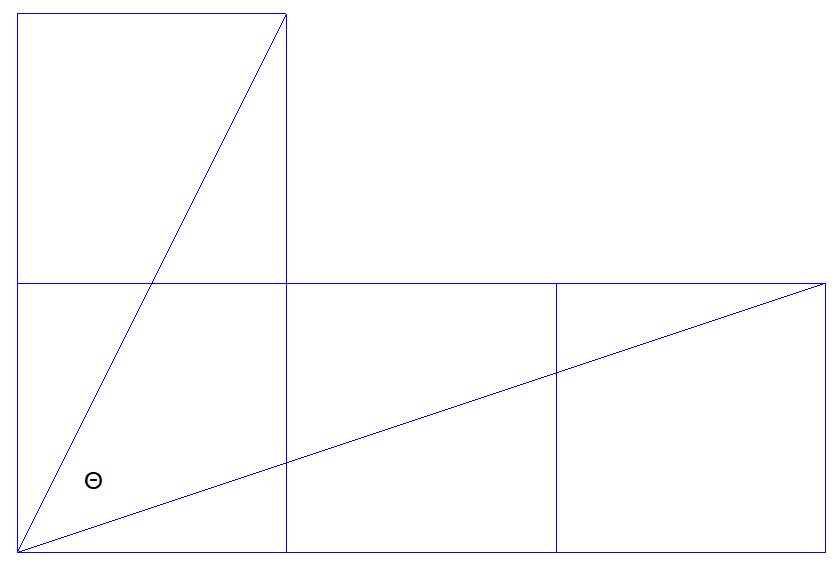
\includegraphics[width=.8\linewidth]{originalTheta.png}
\end{center}

\section*{Solution}
To begin, a Cartesian Plane is superimposed over the original diagram given alongside the challenge. Assume that the bottom left corner to be the origin in this paper

Next, assume the side length of each square to be some constant variable $x$.

\pagebreak

Utilizing this approach, a continuous function can be generated based on the line segments. A simple approach using the definition of slope as rise over yields the equations below:
 Segment 1: $$ y=2x$$
 Segment 2: $$  y=\frac{1}{3}x$$
\begin{center}
	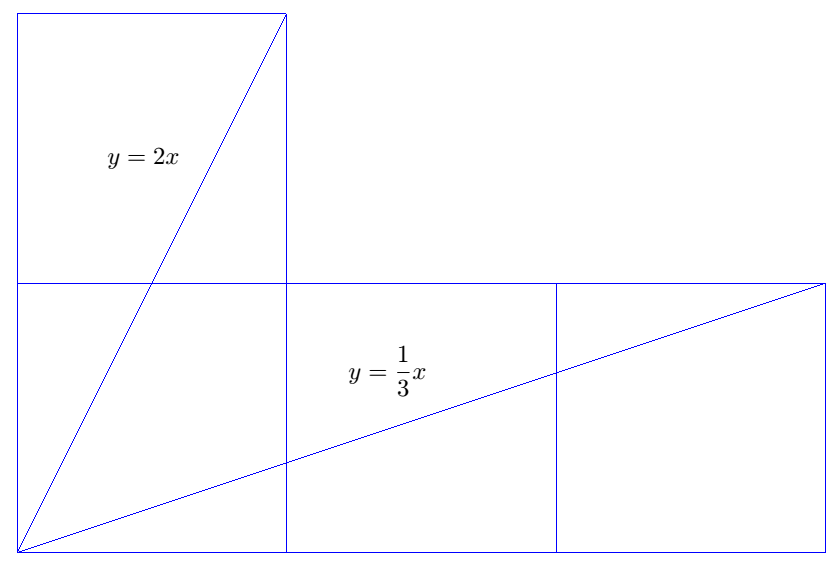
\includegraphics[width=.8\linewidth]{equations.png}
\end{center}

Now, impose a circle with radius $r$ $$x^2+y^2=r^2$$
\begin{center}
	\includegraphics[width=.8\linewidth]{circle.png}
\end{center}

\pagebreak
A chord is created that connects equations 1 and 2. The chord will be referred to as chord $a$. 
\begin{center}
	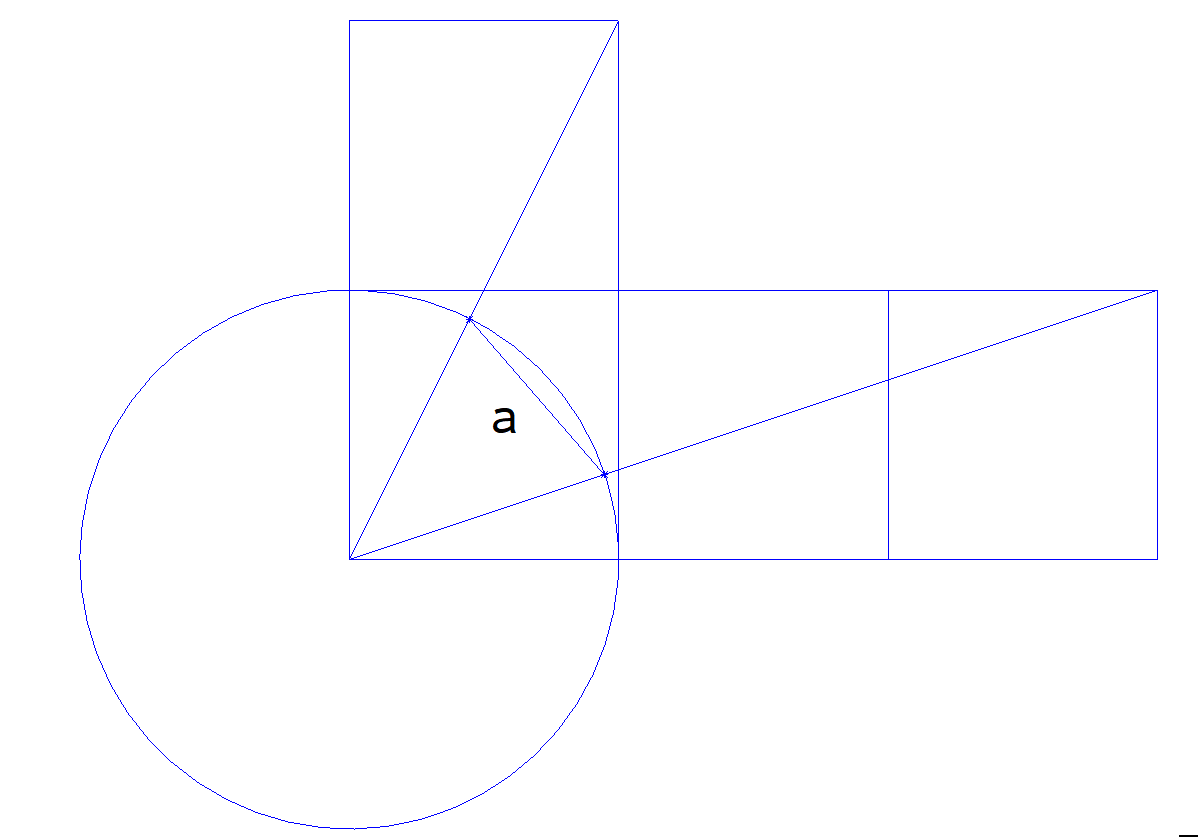
\includegraphics[width=.8\linewidth]{chord.png}
\end{center}

 Utilizing the distance formula, the length of chord a can be found; however, the point of intersections must be found first. To find the points of intersections, use the equation of the circle and the two lines in order to create a system of equations. 
 
$$ y=2x $$
$$ x^2+y^2=r^2 $$

A simple way to solve this system of equations would be to plug in $2x$ for $y$ in the equation of the circle. This yields:

$$ x^2+(2x)^2=r^2 $$

Solving for $x$ gives the $x$-coordinate of one of the intersections.

Using the value of $x$, solve for $y$. 

This yields one point $$\bigg(\frac{ r\sqrt{5} }{5}, \frac{ 2r\sqrt{5} }{5}\bigg)$$

Repeat the same steps, but utilize the other line:
$$ y=\frac{1}{3}x $$
$$ x^2+y^2=r^2 $$

Plug in $\frac{1}{3}x$ for $y$ in the equation of the circle and solve for $x$. Afterwards, using the value of $x$, solve for $y$. 


This yields the point: $$\bigg(\frac{3r\sqrt{10}}{10}, \frac{r\sqrt{10}}{10}\bigg)$$

Now the distance formula can be used to find the length of the chord $a$. Using the points obtained by the system of equations, solve for the length of $a$. 

$$ a=\sqrt{\bigg(\frac{ r\sqrt{5} }{5}-\frac{3r\sqrt{10}}{10}\bigg)^2 + \bigg(\frac{ 2r\sqrt{5} }{5}-\frac{r\sqrt{10}}{10}\bigg)^2}$$


To avoid confusion, do not simplify this solution right way. Instead, continue on and utilize the Law of Cosines.

$$ a^2=b^2+c^2-2bccos\theta$$

Put the value for the length of a and square it to obtain $a^2$. $b$ and $c$ are merely placeholders for the value of the radius which is a length of $r$. This yields $r^2$ for both $b^2$ and $c^2$. 

Now, solve for $\theta$:

$$\bigg(\frac{ r\sqrt{5} }{5}-\frac{3r\sqrt{10}}{10}\bigg)^2 + \bigg(\frac{ 2r\sqrt{5} }{5}-\frac{r\sqrt{10}}{10}\bigg)^2 = 2r^2-2r^2\cos(\theta)$$

 \begin{center}

\includegraphics[width=.8\linewidth]{solution.png}
 \end{center}
Simplifying this yields:
$$\theta=45^o$$
\pagebreak
\section*{Conclusion}

This solution is one of numerous possible solutions to obtaining the angle. Some possible other routes may be to utilize other shapes including squares and rhombi to evaluate theta. Other geometric properties can also be potentially applied to discover the vast array of solutions. 
\end{document}
